\documentclass{article}

% Language setting
% Replace `english' with e.g. `spanish' to change the document language
\usepackage[english]{babel}

% Set page size and margins
% Replace `letterpaper' with `a4paper' for UK/EU standard size
\usepackage[letterpaper,top=2cm,bottom=2cm,left=3cm,right=3cm,marginparwidth=1.75cm]{geometry}

% Useful packages
\usepackage{amsmath}
\usepackage{graphicx}
\usepackage[colorlinks=true, allcolors=blue]{hyperref}
\usepackage{float}
\usepackage{caption}
\usepackage{subfigure}

\title{lab02: Association Analysis -1}
\author{Group 18}


\begin{document}
\maketitle

\section{SimpleKmeans and association analysis}
\subsection{Prepocess and clustering}

This time, we will work with dataset "IRIS", which contains 150 samples and 50 for each 3 classes(Iris setosa, Iris virginica and Iris versicolor), with other 4 different features(the length and the width of sepal and petal).
First, we discretize each of those 4 features into 3 bins, and apply the Kmeans clustering into 3 clusters. We can see that the incorrect clustered rate 6\% which implies that it’s a decent clustering.\\  
\\
Classes to Clusters:\\
\\
  0  1  2  $<$-- assigned to cluster  \\
  0  0 50 | Iris-setosa  \\
 48  2  0 | Iris-versicolor \\
  7 43  0 | Iris-virginica\\
\\
Cluster 0 $<$-- Iris-versicolor  \\
Cluster 1 $<$-- Iris-virginica \\ 
Cluster 2 $<$-- Iris-setosa \\ 
\\
Incorrectly clustered instances :	9.0	  6      \% 

\subsection{Association analysis}

Then we apply association analysis with apriori algorithm by default properties. From the result\ref{fig:apriori_default} we can see that the rules we find are in general different combinations of “class=Iris-setosa”, “petalwidth='(-inf-0.9]'” and “petallength='(-inf-2.966667]' 50”. From visualization\ref{fig:visual_pelenVSpewid} of the discretized data, we can show that for the Iris-setosa(blue datapoints), all datapoint belongs to the above shown petalwidth and petallength bins, and vise versa, within this combination of bins, there is only Iris-setosa. That is why the rules we have are all based on this cluster. It will always have a large support(50, total amount of each class) with confidence 1 whatever the combination or order is. And from the same plot we can expect that this 2 attributes can help a lot when analyzing other 2 classes/clusters too.

\begin{figure}[H]
\centering
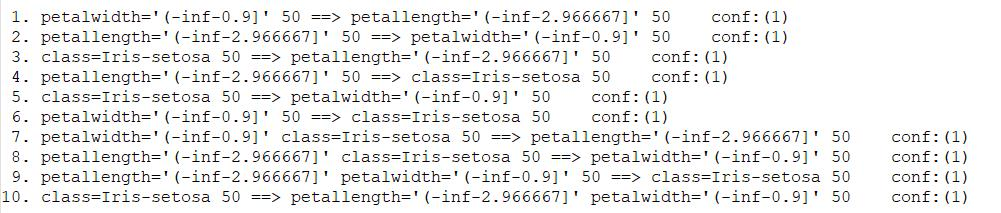
\includegraphics[width=1\textwidth]{apriori_default.jpg}
\caption{\label{fig:apriori_default}best rules under bin=3}
\end{figure}

\begin{figure}[H]
\centering
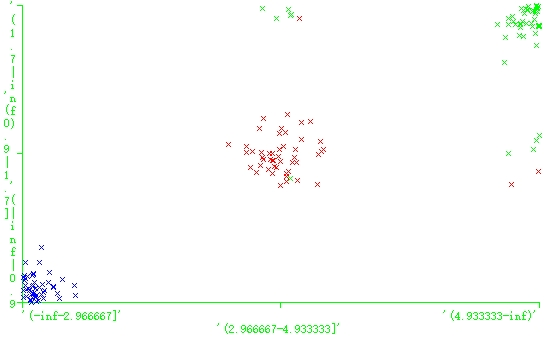
\includegraphics[width=0.8\textwidth]{visual_pelenVSpewid.jpg}
\caption{\label{fig:visual_pelenVSpewid}visualization of petallength vs petalwidth under bin=3\\ color = classes}
\end{figure}

Then we add the cluster we got by SimpleKmeans as an attribute and make it as classindex, then doing association analysis again. But this time the cluster index is from 1-3 instead of 0-2, as shown in the plot\ref{fig:visual_addcluster}.


\begin{figure}[H]
\centering
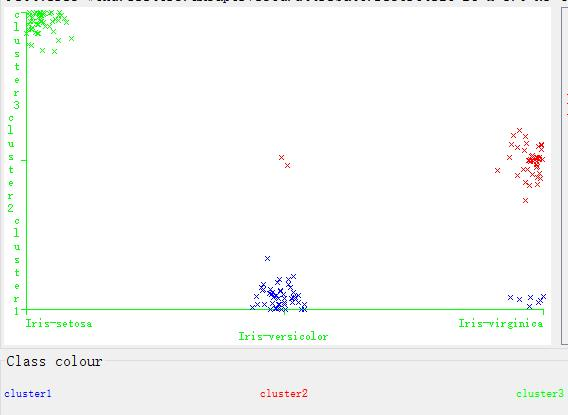
\includegraphics[width=0.8\textwidth]{visual_addcluster.jpg}
\caption{\label{fig:visual_addcluster}visualization of classes vs clusters under bin=3}
\end{figure}


Here are some of the rules we get:\\
\\
petallength='(-inf-2.966667]' petalwidth='(-inf-0.9]' 50 ==$>$ cluster=cluster3 50    conf:(1)\\


The same as what we discussed, the Iris-setosa are all clustered in to cluster3 and easily found by the Apriori algorithm.
\\
petallength='(2.966667-4.933333]' petalwidth='(0.9-1.7]' 48 ==$>$ cluster=cluster1 48    conf:(1)\\
petallength='(4.933333-inf)' petalwidth='(1.7-inf)' 40 ==$>$ cluster=cluster2 40    conf:(1)\\

Similarly, this two attributes made rules towards cluster1\&2 as we expected. With a high support along with high confidence.

\section{Association analysis with HierarchicalClusterer }

\begin{figure}[H]
\centering
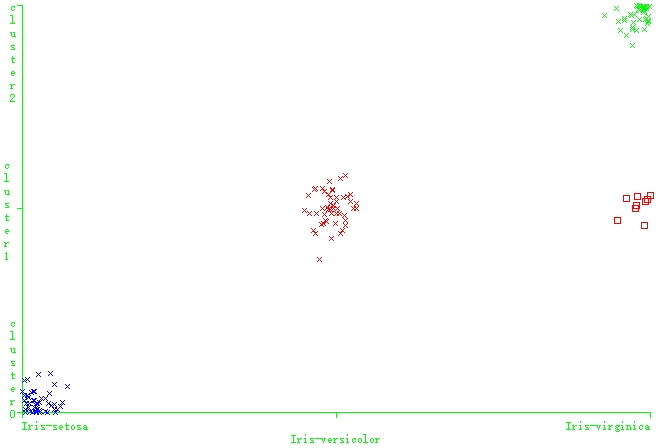
\includegraphics[width=0.8\textwidth]{hierarchical_classVScluster.jpg}
\caption{\label{fig:hierarchical_classVScluster}visualization of classes vs clusters under bin=3 with HierarchicalClusterer\\color = clusters}
\end{figure}

Then with the same discretized dataset, we apply HierarchicalClusterer with average distance as clustering algorithm, and we get a little bit different clustering result\ref{fig:hierarchical_classVScluster} and add it as an attribute. Then do the association analysis with these new cluster labels. Here are some of the rules we found:\\
\\
petallength='(2.966667-4.933333]' 54 ==$>$ cluster=cluster2 54    conf:(1) \\
petallength='(-inf-2.966667]' petalwidth='(-inf-0.9]' 50 ==$>$ cluster=cluster1 50    conf:(1)\\
petallength='(4.933333-inf)' petalwidth='(1.7-inf)' 40 ==$>$ cluster=cluster3 40    conf:(1)\\
\\

Again for the same reason as it was in previous Kmeans clustering, those 2 attributes petallength and petalwidth made association rules with the best support and confident. Under the 3-bin discretization method we are using, those bins already did a preprocess job of collecting different continuous values into one same discrete bin and made the clustering easier to get similar results, and thus so do the association analysis. We can expect that the results we get will differ greater if we do the clustering before discretize or use different number of bins to discretize.

\section{Association analysis with discretization under bin = 9}

Now we discretize the data by bin = 9, then do the kmeans clustering. This time the clustering result is not so favorable. The main issue is that a large portion of Iris-virginica was wrongly clustered into the cluster of Iris-versicolor.\\
\\
Classes to Clusters:\\
\\
  0  1  2  $<$-- assigned to cluster\\
  1  1 48 | Iris-setosa\\
 43  3  4 | Iris-versicolor\\
 24 26  0 | Iris-virginica\\
\\
Cluster 0 $<$-- Iris-versicolor\\
Cluster 1 $<$-- Iris-virginica\\
Cluster 2 $<$-- Iris-setosa\\
\\
Incorrectly clustered instances :	33.0	 22      \% \\
\\

Then again we do the association analysis, here are some of the rules we found:\\
\\
petallength='(-inf-1.655556]' petalwidth='(-inf-0.366667]' 38 ==$>$ cluster=cluster3 38    conf:(1)\\
petalwidth='(1.166667-1.433333]' 26 ==$>$ cluster=cluster1 26    conf:(1)\\
sepallength='(6.3-6.7]' 22 ==$>$ cluster=cluster2 16    conf:(0.73)\\
\\

From these rules we can find that for cluster2, the used-to-be credible petallength\&petalwidth features no longer works well, the best rule of cluster2 is using sepallength as antecedent. From the visualization\ref{fig:bin9_pelenVSepwid} of petallength and petalwidth we can see that the clustering shown in this plot is not as distinct as is was when we discretize by bin = 3.

\begin{figure}[H]
\centering
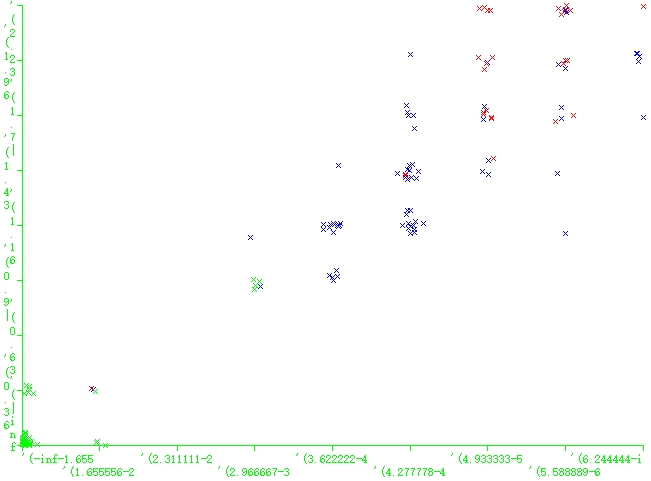
\includegraphics[width=0.8\textwidth]{bin9_pelenVSepwid.jpg}
\caption{\label{fig:bin9_pelenVSepwid}visualization of petallenth vs petalwidth under bin=9\\color = clusters}
\end{figure}

From all the results above we can conjecture that it’s the discretization merge too much datapoints of different classes into one same bin, which makes the clustering algorithm cannot separate them. And the dimension of features makes the situation worse. As a result, nearly half of the Iris-virginica was forced encompassed into the cluster of Iris-versicolor. Seems discretize by 3 bins is some kind of the real important prior knowledge based on class label and corresponding distribution of features we already known that helps us getting a good clustering and association result.



\end{document}